\documentclass{gdl}

\usepackage[T1]{fontenc} 
\usepackage[utf8]{inputenc} 
\usepackage{lmodern} 
\usepackage{graphicx} 
\usepackage{hyperref} 
\usepackage{geometry} 
\usepackage{longtable} 
\usepackage{tcolorbox}
\usepackage{booktabs} 
\usepackage{textcomp} 
\usepackage{fontawesome5} 
\usepackage{array} 
\usepackage{enumitem}
\usepackage{tocloft}
\usepackage{float}

% CHANGE THESE
\def\groupid{------}
\def\projectid{------}

\setlength{\parindent}{0pt}
\begin{document}

% CHANGE THIS
\title{Linear Transformer Topological Masking with Graph Random Features}

% CHANGE THIS
\author{%
Paolo Deidda, Raffaele Perri, Paul Leopold Seipl\\
\texttt{\{paolo.deidda, raffaele.perri, paul.leopold.seipl\}@usi.ch}
}

\begin{abstract}
Concise and self-contained description of your project, motivation and main findings.
\end{abstract}

\maketitle
\vfill
\tableofcontents

\newpage

\twocolumn

% ==========================================================================
% ==========================================================================
\section{Introduction}

Transformers have established themselves as a dominant architecture across various machine learning modalities, deriving their power from the attention mechanism which models complex dependencies between tokens \cite{vaswani2017attention}. However, the standard Transformer treats input data as a set, making it invariant to permutation and inherently unaware of structural dependencies, such as the connectivity in graph-structured data. To address this, \textit{Topological Masking} is often employed, where the attention mechanism is modulated by a function of the graph structure (e.g., shortest path distance or adjacency), injecting a necessary structural inductive bias \cite{ying2021do, choromanski2022rethinking}.

A fundamental computational conflict arises when scaling this approach to large graphs. Standard ``Vanilla'' Softmax attention requires explicitly computing and storing an $N \times N$ attention matrix, resulting in quadratic $\mathcal{O}(N^2)$ time and space complexity. While Linear Attention mechanisms address this bottleneck by leveraging low-rank decompositions $\phi(Q)(\phi(K)^T V)$ to achieve $\mathcal{O}(N)$ complexity \cite{katharopoulos2020transformers}, they rely strictly on the associativity of matrix multiplication. Introducing a topological mask $M$ generally breaks this associativity—since $(A \times B) \odot M \neq A \times (B \odot M)$—forcing the re-materialization of the dense attention matrix and negating the efficiency gains of linear attention.

In this work, we focus on the reproduction of ``Linear Transformer Topological Masking with Graph Random Features'' \cite{reid2025linear}. The authors propose a novel solution to the masking conflict by approximating the topological mask using Graph Random Features (GRFs). By decomposing the mask into sparse feature vectors derived from random walks, the method allows the mask to be fused with query and key features via a tensor product, preserving the $\mathcal{O}(N)$ complexity of linear attention while maintaining the expressivity of topological masking.

\begin{figure}[h]
    \centering
    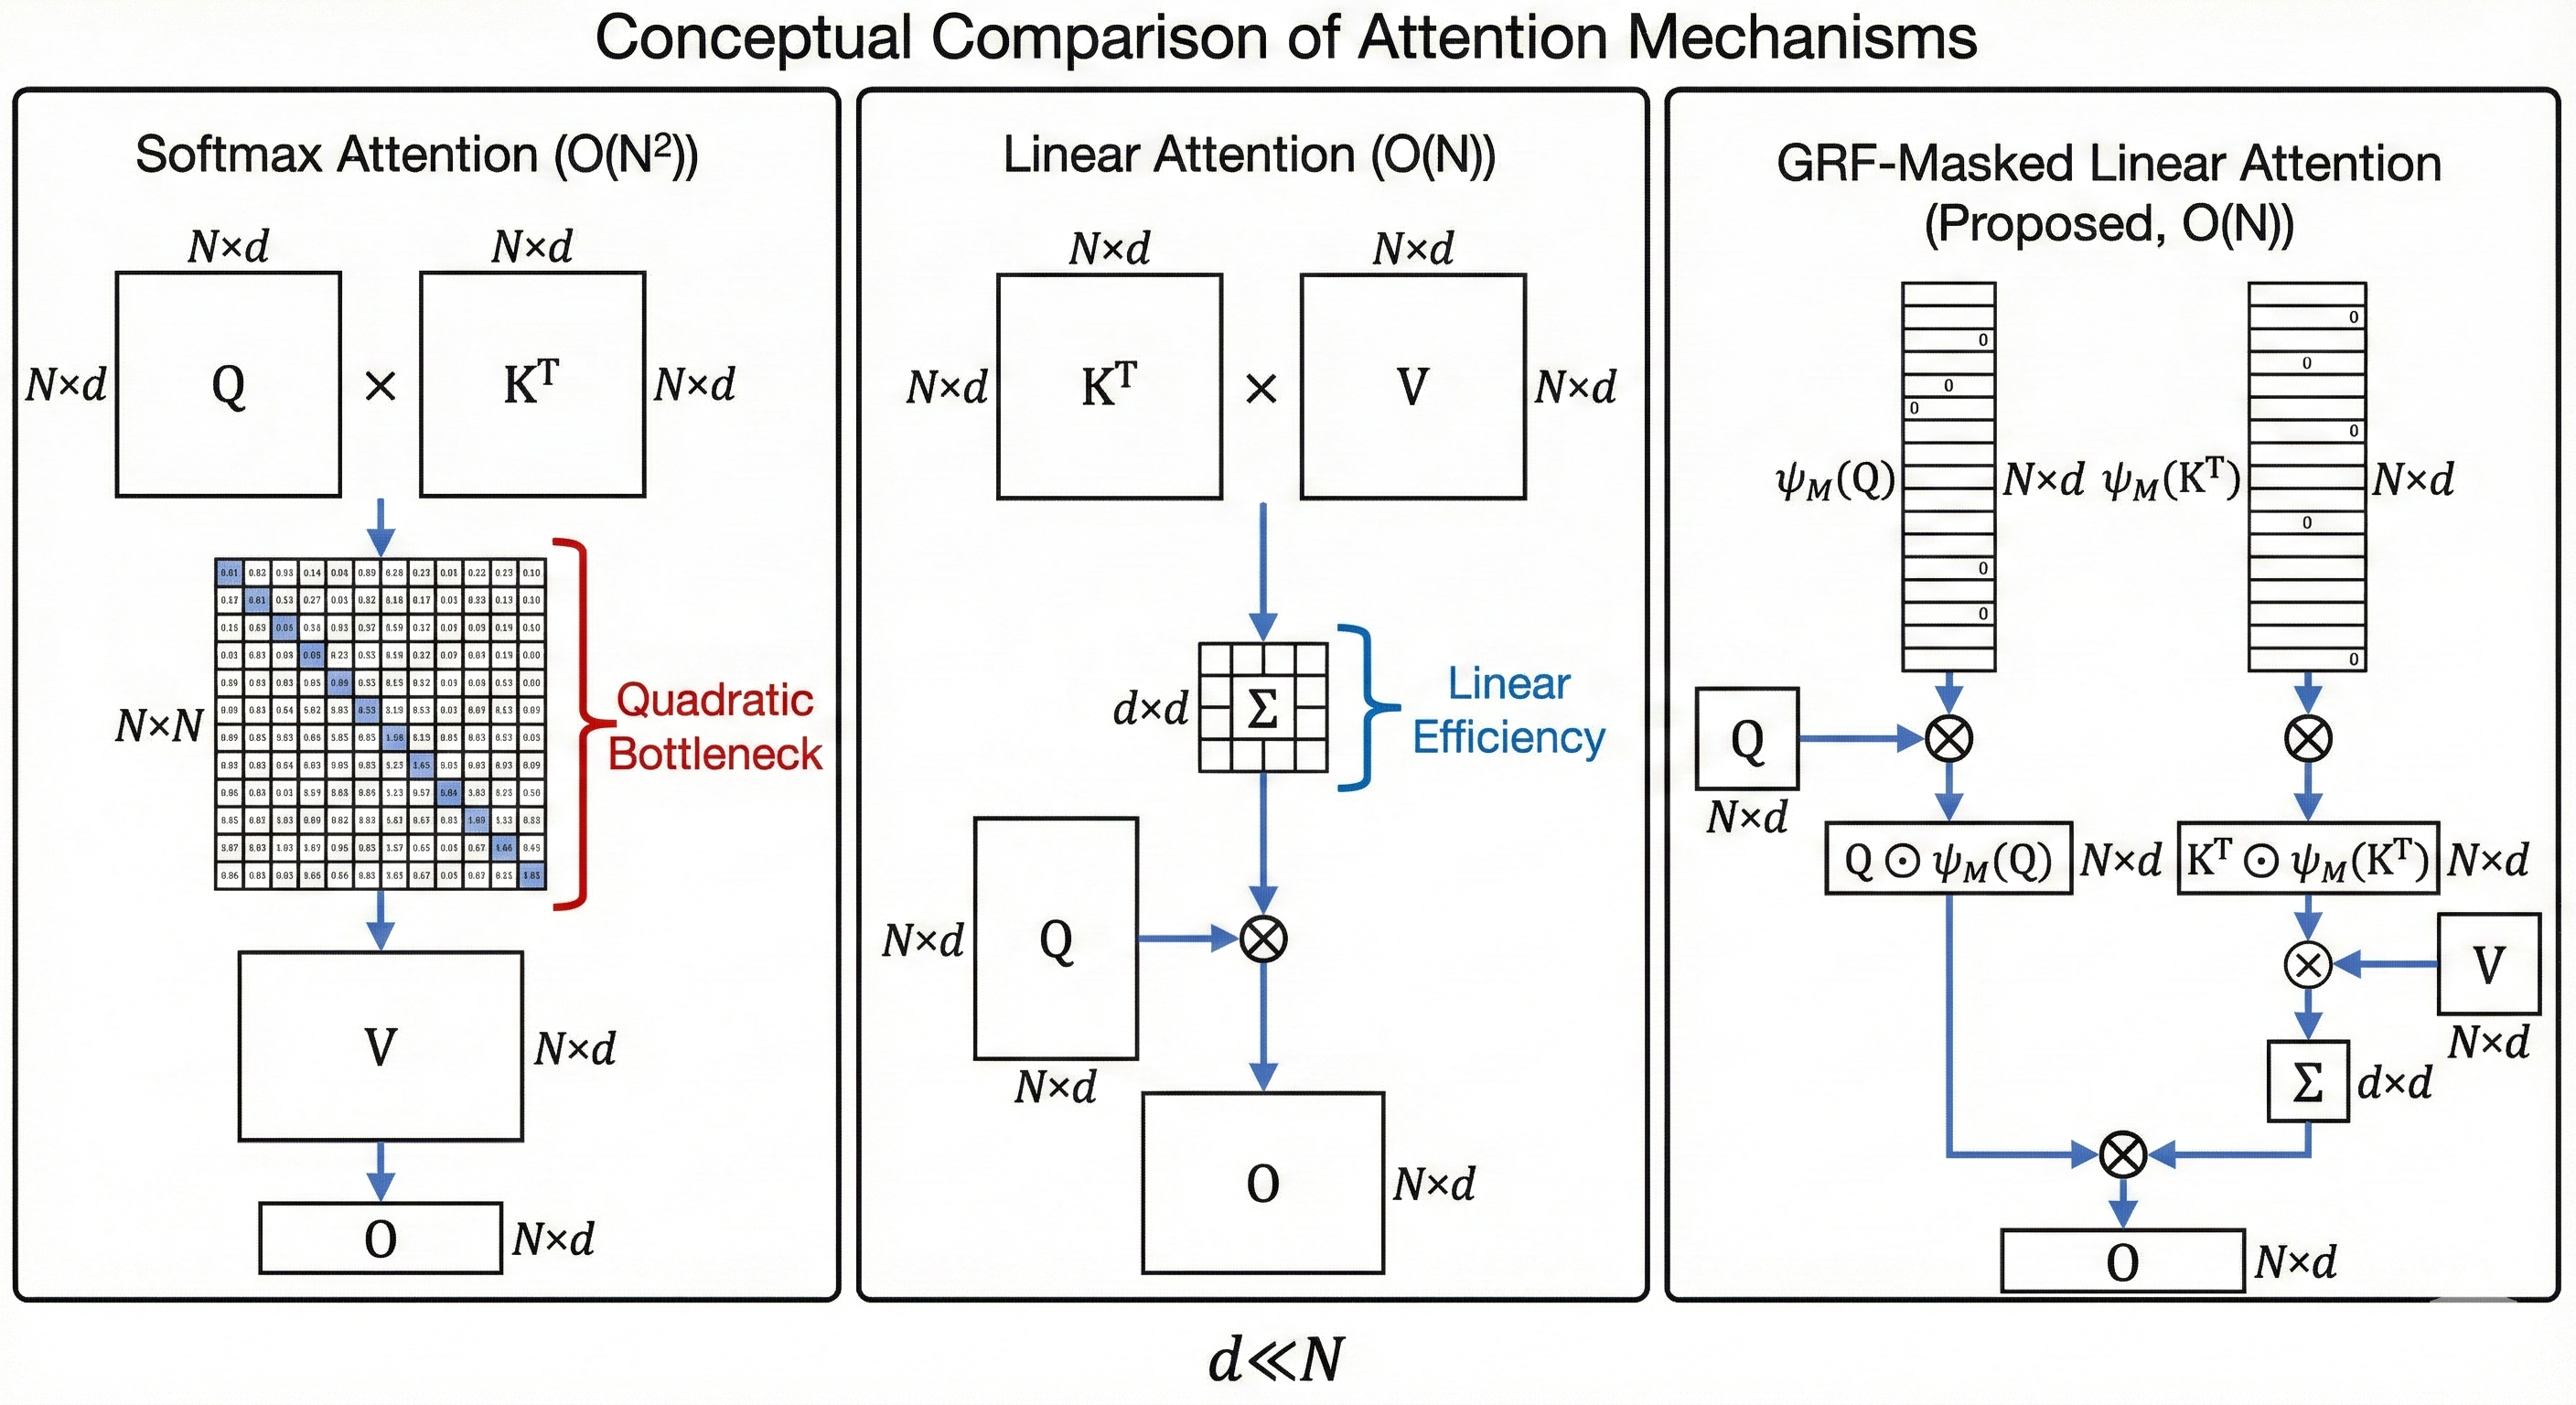
\includegraphics[width=\linewidth]{assets/schematic_overview.png}
    \caption{Conceptual comparison of attention mechanisms. The left panel illustrates the quadratic bottleneck of Softmax attention. The middle panel shows the efficient flow of Linear attention. The right panel demonstrates the proposed GRF method, which preserves linear complexity by fusing sparse topological features $\psi_M$ with the query/key representations.}
    \label{fig:attention_comparison}
\end{figure}

\paragraph{Contributions and Replication Results}
Our primary contribution is a validation of the theoretical and empirical claims presented in the original paper. We successfully implemented the proposed GRF-based masking mechanism and conducted a rigorous analysis of its computational scaling behavior.

\begin{itemize}
    \item \textbf{Time Complexity Verification:} We replicated the scaling experiment comparing Softmax, Linear, and GRF-Masked attention. Our results confirm the theoretical claims: while Softmax attention scales quadratically, exhibiting a ``computational explosion'' for $N > 8$, the GRF-Masked method maintains strict linear scaling $\mathcal{O}(N)$.
    
    \item \textbf{Overhead Analysis:} We quantified the overhead introduced by the GRF mechanism. While retaining the linear complexity class, we observe a constant factor increase in FLOPs compared to unmasked linear attention, attributable to the sparsity of the generated graph features.
\end{itemize}

\textbf{!!!TO DO: ADD THE OTHER TWO EXPERIMENTS RESULTS OVERVIEW!!!}
% ==========================================================================
% ==========================================================================
\section{Related works}

\subsubsection{Standard and Topological Attention}
The standard self-attention mechanism, introduced by \cite{vaswani2017attention}, computes a dense $N \times N$ attention matrix $A = \text{softmax}(QK^\top / \sqrt{d})$. While highly effective at modeling global dependencies, this approach incurs quadratic $\mathcal{O}(N^2)$ time and space complexity, prohibiting its use on long sequences or large graphs.
To adapt Transformers to graph-structured data, \textit{topological masking} is often employed to inject structural inductive bias \cite{ying2021do}. This typically involves modulating the attention scores with a mask $M(\mathcal{G})$ derived from the graph topology (e.g., shortest path distances), forcing tokens to attend preferentially to their structural neighbors. However, applying such masks generally requires materializing the full $N \times N$ matrix, maintaining the prohibitive quadratic bottleneck.

\subsubsection{Linear Attention and The Masking Conflict}
To address the scalability limits of standard attention, \textit{Linear Attention} mechanisms have been proposed \cite{katharopoulos2020transformers, choromanski2020rethinking}. These methods replace the softmax kernel with a feature map decomposition $\phi(\cdot)$, allowing the computation to be reordered via associativity: $D^{-1}\phi(Q)(\phi(K)^\top V)$. This reduces complexity to $\mathcal{O}(N)$.
However, as noted in the foundational literature, introducing an element-wise topological mask $M$ breaks this associativity, i.e., $(A \times B) \odot M \neq A \times (B \odot M)$. Consequently, standard linear attention methods are generally incompatible with flexible topological masking without reverting to quadratic complexity.

\subsubsection{Efficient Masking Approaches}
Several approaches have attempted to reconcile efficiency with masking, though often with restrictions on graph topology.
\cite{luo2021stable} and \cite{choromanski2022rethinking} proposed using Toeplitz matrices and the Fast Fourier Transform (FFT) to implement masking in $\mathcal{O}(N \log N)$ time. While an improvement over $\mathcal{O}(N^2)$, these methods are largely restricted to highly structured graphs like grids or trees and do not generalize easily to arbitrary topologies.
Other methods, such as stochastic positional encoding \cite{liutkus2021relative}, achieve linear complexity but are similarly limited to sequence data (1D grids).
The method reproduced in this work \cite{reid2025linear} distinguishes itself by supporting general graphs with strict $\mathcal{O}(N)$ complexity via a randomized low-rank decomposition of the mask itself.
% ==========================================================================
% ==========================================================================
\section{Methodology}

% Experiment 4.1 and 4.3 — Time Complexity & Ablation Studies
\subsection{Time Complexity}
To validate the theoretical efficiency claims of the proposed architecture, the paper conducts a hardware-agnostic analysis of computational cost. Instead of measuring wall-clock time, which can be conflated by hardware specifics (GPU/CPU differences) and implementation overhead, the methodology focuses on counting the total number of Floating Point Operations (FLOPs) required for a single forward pass of the attention mechanism.\\
The analysis compares three distinct attention variants across a range of graph sizes (N):
\begin{itemize}
    \item \textbf{Unmasked Softmax Attention:} The standard $\mathcal{O}(N^2)$ mechanism, where the full N×N attention matrix is materialized.
    \item \textbf{Unmasked Linear Attention:} An $\mathcal{O}(N)$ efficient alternative that utilizes a low-rank decomposition $\phi(Q)(\phi(K)^T V)$.
    \item \textbf{GRF-Masked Linear Attention (Ours):} The proposed method, which approximates the topological mask using Graph Random Features. While theoretically $\mathcal{O}(N)$, this method involves constructing sparse feature matrices, introducing a constant overhead dependent on the graph sparsity and number of random walkers.
\end{itemize}
The theoretical FLOP counts are derived based on the matrix dimensions involved. For a hidden dimension $d$ and feature dimension $m$:
\begin{itemize}
    \item \textbf{Softmax Attention (Baseline):} Dominated by the $N^2$ term from $QK^\top$ and $AV$ product, roughly scaling as $\mathcal{O}(4N^2d)$.
    \item \textbf{Linear Attention (Unmasked):} Linear in $N$, scaling as  $\mathcal{O}(4Nmd)$ due to the associativity of matrix multiplication.
    \item \textbf{GRF-Masked Linear Attention (Ours):} Also linear in $N$, but the exact cost depends on the number of non-zero entries (NNZ) in the sparse graph random feature vectors. The complexity scales as $\mathcal{O}(4 \cdot \text{NNZ} \cdot d)$.
\end{itemize}
The experiment uses a 1-dimensional grid graph (a linear chain) to test scaling behavior. This topology allows for controlled testing of "local" attention, as the number of neighbors remains constant as $N$ increases.

% Experiment 4.2 — VITS (Vision Image Topological Sampling): Vision–Image Tasks (Graph + Image Integration)
\subsection{VITS: Vision--Image Tasks (Graph + Image Integration)}

% Experiment 4.4 — PCTS (Point Cloud Temporal State prediction): Predicting Particle Cloud Temporal States
\subsection{PCTS: Point Cloud Temporal State prediction}


% ======================== previous content ========================
% ==================================================================

% \textit{You can change the name of this section as you see fit.}\\
% In this section you should give a description of the methodological aspects of your work, for instance how you modified an existing method to perform a particular task or to overcome a particular limitation. If your project is about reproducibility, here you should describe the method presented in the original paper.


% ==========================================================================
% ==========================================================================
\section{Implementation}

% Experiment 4.1 and 4.3 — Time Complexity & Ablation Studies
\subsection{Time Complexity \& Ablation Studies}

% Experiment 4.2 — VITS (Vision Image Topological Sampling): Vision–Image Tasks (Graph + Image Integration)
\subsection{VITS: Vision--Image Tasks (Graph + Image Integration)}

% Experiment 4.4 — PCTS (Point Cloud Temporal State prediction): Predicting Particle Cloud Temporal States
\subsection{PCTS: Point Cloud Temporal State prediction}





% ======================== previous content ========================
% ==================================================================

% This section should be structured as follows (from the Reproducibility challenge template):

% ---

% Briefly describe what you did and which resources did you use. E.g. Did you use author's code, did you re-implement parts of the pipeline, how much time did it take to produce the results, what hardware you were using and how long it took to train/evaluate. 

% \subsection{Datasets}
% Describe the datasets you used and how you obtained them. 

% \subsection{Hyperparameters}
% Describe how you set the hyperparameters and what was the source for their value (e.g. paper, code or your guess). 

% \subsection{Experimental setup}
% Explain how you ran your experiments, e.g. the CPU/GPU resources and provide the link to your code and notebooks.

% \subsection{Computational requirements}
% Provide information on computational requirements for each of your experiments. For example, the number of CPU/GPU hours and memory requirements. You'll need to think about this ahead of time, and write your code in a way that captures this information so you can later add it to this section. 

% ==========================================================================
% ==========================================================================
\section{Results}

% Experiment 4.1 and 4.3 — Time Complexity & Ablation Studies
\subsection{Time Complexity \& Ablation Studies}

% Experiment 4.2 — VITS (Vision Image Topological Sampling): Vision–Image Tasks (Graph + Image Integration)
\subsection{VITS: Vision--Image Tasks (Graph + Image Integration)}

% Experiment 4.4 — PCTS (Point Cloud Temporal State prediction): Predicting Particle Cloud Temporal States
\subsection{PCTS: Point Cloud Temporal State prediction}


% ======================== previous content ========================
% ==================================================================

% In this section you should report the results of your work (e.g., the outcome of an empirical analysis). You should be objective and support your statements with empirical evidence.

% \begin{table}[h]
% \small\sf\centering
% \caption{Experimental results (average of 3 runs).}
% \begin{tabular}{l c c}
% \toprule
% Methods & MAE & MSE\\
% \midrule
% \texttt{Baseline1} & $21.23 \pm 1.65$ & $841.36 \pm 12.65$\\
% \texttt{Baseline2} & $15.45 \pm 1.02$ & $652.38 \pm 09.89$\\
% \midrule
% \texttt{Method} & $12.03 \pm 0.35$ & $324.13 \pm 05.56$\\
% \bottomrule
% \end{tabular}
% \label{tab:table}
% \end{table}

% Use figures, plots and tables (like \autoref{tab:table}) to present your results in a nice and readable way.


% ==========================================================================
% ==========================================================================
\section{Discussion and conclusion}
\subsection{Time Complexity}
\subsection{Vision Transformers (ViTs)}
\subsection{PCTS: Point Cloud Temporal State prediction}
\subsection{Conclusion}
% ==========================================================================
% ==========================================================================
% Bibliography
\onecolumn
\bibliography{bibliography}
\bibliographystyle{unsrtnat}
\clearpage

\end{document}
